\clearpage
\makeatletter
\efloat@restorefloats
\makeatother


\begin{appendix}
\section{}
\hypertarget{s1}{%
\subsection{S1: Experiments included in the linear mixed-effects
model}\label{s1}}

The selected experiments consist of an artificial grammar learning task
with 12-month-old infants. These experiments are characterized by
variability in the number of infants' prior HPP visits\footnote{At the
  time of publication of Saffran \& Wilson (2003), the first author
  noted that there appeared to be an association between the number of
  prior studies completed by the infants and the direction of
  preference. The analysis was included in the original manuscript
  submission but was removed from later revisions based on reviewer
  suggestions.}. They include all studies run in the two senior authors'
labs that included (a) 11- to 13-month-old participants; (b) HPP; (c)
artificial grammar learning (linguistic or non-linguistic); (d) 2 to 5
minutes of exposure; (e) an \emph{a priori} hypothesis that infants
would show learning; (f) visit numbers recorded at the time of testing.
The studies are thus as well matched as is possible given the
retrospective nature of this analysis.

\emph{Saffran \& Wilson (2003)} demonstrated that 12-month-old infants
can compute multiple regularities from a finite-state grammar. Infants
were able to first segment words from running speech based on
transitional probabilities, then detect permissible orderings of the
segmented words. Test items consisted of grammatical and ungrammatical
sentences that could only be discriminated based on word-level
information (transitional probabilities between syllables were not
informative about the ``grammaticality'' of test items). Infants showed
a significant familiarity preference: \emph{F}(1, 38)= 5.37, \emph{p}
\textless{} .05.

\emph{Saffran, Hauser, Seibel, Kapfhamer, Tsao, \& Cushman (2008)}
demonstrated that infants could detect simple phrases (i.e., clusters of
nonsense words grouped together based on statistical regularities) from
artificial grammars. In Exp. 1, infants in the Predictive Language
condition were familiarized with a grammar including predictive
(statistical) dependencies between words. The test items consisted of
familiar sentences vs.~novel sentences violating the grammar. Infants
showed a significant novelty preference: \emph{t}(11) = 2.52, \emph{p}
\textless{} .05.

\emph{Santolin \& Saffran (2019)} is a conceptual replication of Saffran
et al. (2008) using non-linguistic sounds (e.g., computer alert sounds)
to implement the grammars. Infants exposed to the Predictive language
showed a significant novelty preference: \emph{t}(26) = 2.45, \emph{p} =
.021, \emph{d} = 0.47.

We replicated the Predictive Language condition of Santolin \& Saffran
(2019) at the University Pompeu Fabra, Barcelona (\emph{Santolin,
Saffran \& Sebastian-Galles, 2019}, 2019), using identical stimuli and
procedures. We found significant discrimination of the test stimuli but
observed the opposite direction of preference: infants listened longer
to familiar than novel strings: \emph{t}(23) = 2.30, \emph{p} = .030,
\emph{d} = 0.47. All results are shown in Figure 1 of the main
manuscript.

\hypertarget{s2}{%
\subsection{S2: Participants information}\label{s2}}

We retrieved data from 102 infants who had participated in a range of
1-6 HPP visits. Three of the experiments were run in Madison, WI
(University of Wisconsin-Madison): Saffran \& Wilson, 2003 (Exp. 2;
\emph{N}=40, mean age: 11.5 months); Saffran et al., 2008 (Exp. 1,
Condition P-Language: \emph{N}=12, mean age: 12.8 months); Santolin \&
Saffran, 2019 (Condition 1; \emph{N}=26, mean age: 12.9 months). One
study was run in Barcelona, Spain (Universitat Pompeu Fabra): Santolin,
Saffran \& Sebastian-Galles, 2019 (\emph{N}=24, mean age: 13 months).
All studies were conducted according to guidelines provided by the
Declaration of Helsinki, with written informed consent obtained from a
caregiver for each child before any assessment or data collection.
Ethical approval was granted by the University of Wisconsin-Madison
Social and Behavioral Sciences IRB for Saffran \& Wilson (2003), Saffran
et al. (2008), and Santolin \& Saffran (2019), and by the Comitè Etic
d'Investigació Clinica, Parc de Salut Mar Barcelona, for Santolin et al.
(2019).

Two data points (average looking time for familiar and novel test items)
were available for each participant. Participants included in the
current analysis are those included in the final version of the studies.

\hypertarget{s3}{%
\subsection{S3: Linear mixed-effects model - additional
information}\label{s3}}

We fit a model predicting looking time (\(LT\)) including \(Item\)
(Familiar vs.~Novel), number of Head-turn Preference Procedure
experiments completed by infants (\(HPP\)), and their interaction
(\(Item \times HPP\)) as fixed effects. Participant and study {[}4
levels: Santolin \& Saffran (2019), Santolin, Saffran \&
Sebastian-Galles (2019), Saffran et al.~(2008), Saffran \& Wilson
(2003){]} were included as random effects. Following Barr, Levy,
Scheepers, \& Tily (2013), we fit a model with the maximal random
effects structure including random intercepts by-participant and
by-study, and random slopes of \(HPP\) by-participant and by-study.
However, due to lack of convergence, we pruned the random effects
structure until convergence was achieved (e.g., Brauer \& Curtin, 2018).
The final model included by-participant and by-study random intercepts
only. This model accounts for cross-participant variability in overall
looking time (as some infants look longer than others), and for
cross-study differences in overall looking time. The model was fit using
the \texttt{lme4} R package (Bates, Kliegl, Vasishth, \& Baayen, 2015).
We used the \texttt{Anova} function from the \texttt{car} R package (Fox
\& Weisberg, 2019) to perform \emph{F}-tests on fixed effects using
Kenward-Roger's approximation of the degrees of freedom (e.g., Judd,
Westfall, \& Kenny, 2012).

\hypertarget{s4}{%
\subsection{S4: Results sub-setting data to participants with less than
6, 5, 4, and 3 HPP studies}\label{s4}}

Consistent with the results of the entire dataset, we found a
statistically significant interaction of \emph{Test Item} with the
number of \emph{HPP} visits when reducing the sample to the infants who
participated in less than 6, 5, 4, and 3 HPP experiments. Below, a table
reporting the output of the linear mixed-effects model fitted on the
original and reduced samples.

\begin{longtable}[]{@{}llllllll@{}}
\caption{(\#tab:unnamed-chunk-17)Summary of the results of the linear
mixed-effects model performed on the reduced data.}\tabularnewline
\toprule
\textbf{Subset} & \textbf{Term} & \textbf{Coefficient} &
\textbf{\emph{SEM}} & \textbf{95\% CI} & \textbf{F} & \textbf{Den.
\emph{df}} & \textbf{\emph{p}}\tabularnewline
\midrule
\endfirsthead
\toprule
\textbf{Subset} & \textbf{Term} & \textbf{Coefficient} &
\textbf{\emph{SEM}} & \textbf{95\% CI} & \textbf{F} & \textbf{Den.
\emph{df}} & \textbf{\emph{p}}\tabularnewline
\midrule
\endhead
Original & \emph{Intercept} & 7,679.0 & 673.3 & {[}6389.7, 9294.6{]} &
124.6 & 9.1 & \textless{} .001\tabularnewline
& \emph{Test Item} & -1,398.8 & 411.3 & {[}-2204.9, -589.1{]} & 11.6 &
100.0 & .001\tabularnewline
& \emph{HPP} & -539.7 & 238.7 & {[}-999.9, -74.7{]} & 4.8 & 133.1 &
.030\tabularnewline
& \emph{Test Item \(\times\) HPP} & 667.1 & 192.6 & {[}247.2, 1028.5{]}
& 12.0 & 100.0 & .001\tabularnewline
HPP 1-5 & \emph{Intercept} & 7,675.0 & 691.6 & {[}6452.7, 9029.3{]} &
118.3 & 10.1 & \textless{} .001\tabularnewline
& \emph{Test Item} & -1,416.1 & 435.4 & {[}-2237.7, -543.7{]} & 10.6 &
99.0 & .002\tabularnewline
& \emph{HPP} & -535.6 & 261.2 & {[}-1081.1, -37.5{]} & 4.0 & 133.6 &
.048\tabularnewline
& \emph{Test Item \(\times\) HPP} & 677.8 & 211.3 & {[}241, 1081.9{]} &
10.3 & 99.0 & .002\tabularnewline
HPP 1-4 & \emph{Intercept} & 7,611.1 & 719.3 & {[}6188.6, 9275.3{]} &
107.4 & 10.5 & \textless{} .001\tabularnewline
& \emph{Test Item} & -1,491.1 & 452.1 & {[}-2348.4, -578.5{]} & 10.9 &
98.0 & .001\tabularnewline
& \emph{HPP} & -500.8 & 278.7 & {[}-1070.2, 98.2{]} & 3.0 & 131.9 &
.083\tabularnewline
& \emph{Test Item \(\times\) HPP} & 726.2 & 224.9 & {[}294.2, 1145{]} &
10.4 & 98.0 & .002\tabularnewline
HPP1-3 & \emph{Intercept} & 7,470.0 & 794.6 & {[}6007.1, 9172.6{]} &
83.8 & 14.3 & \textless{} .001\tabularnewline
& \emph{Test Item} & -1,349.9 & 532.3 & {[}-2426.9, -267.6{]} & 6.4 &
92.0 & .013\tabularnewline
& \emph{HPP} & -395.8 & 366.6 & {[}-1182.6, 316.1{]} & 1.1 & 122.3 &
.299\tabularnewline
& \emph{Test Item \(\times\) HPP} & 627.9 & 294.1 & {[}3, 1252.6{]} &
4.6 & 92.0 & .035\tabularnewline
HPP 1-2 & \emph{Intercept} & 7,301.9 & 1009.9 & {[}5253.3, 9362.1{]} &
48.9 & 23.9 & \textless{} .001\tabularnewline
& \emph{Test Item} & -1,783.7 & 726.7 & {[}-3199.6, -360.7{]} & 6.0 &
78.0 & .016\tabularnewline
& \emph{HPP} & -261.3 & 586.8 & {[}-1449.8, 991.7{]} & 0.2 & 107.0 &
.667\tabularnewline
& \emph{Test Item \(\times\) HPP} & 969.5 & 481.8 & {[}38.3, 2010.4{]} &
4.0 & 78.0 & .048\tabularnewline
\bottomrule
\end{longtable}

\begin{figure}
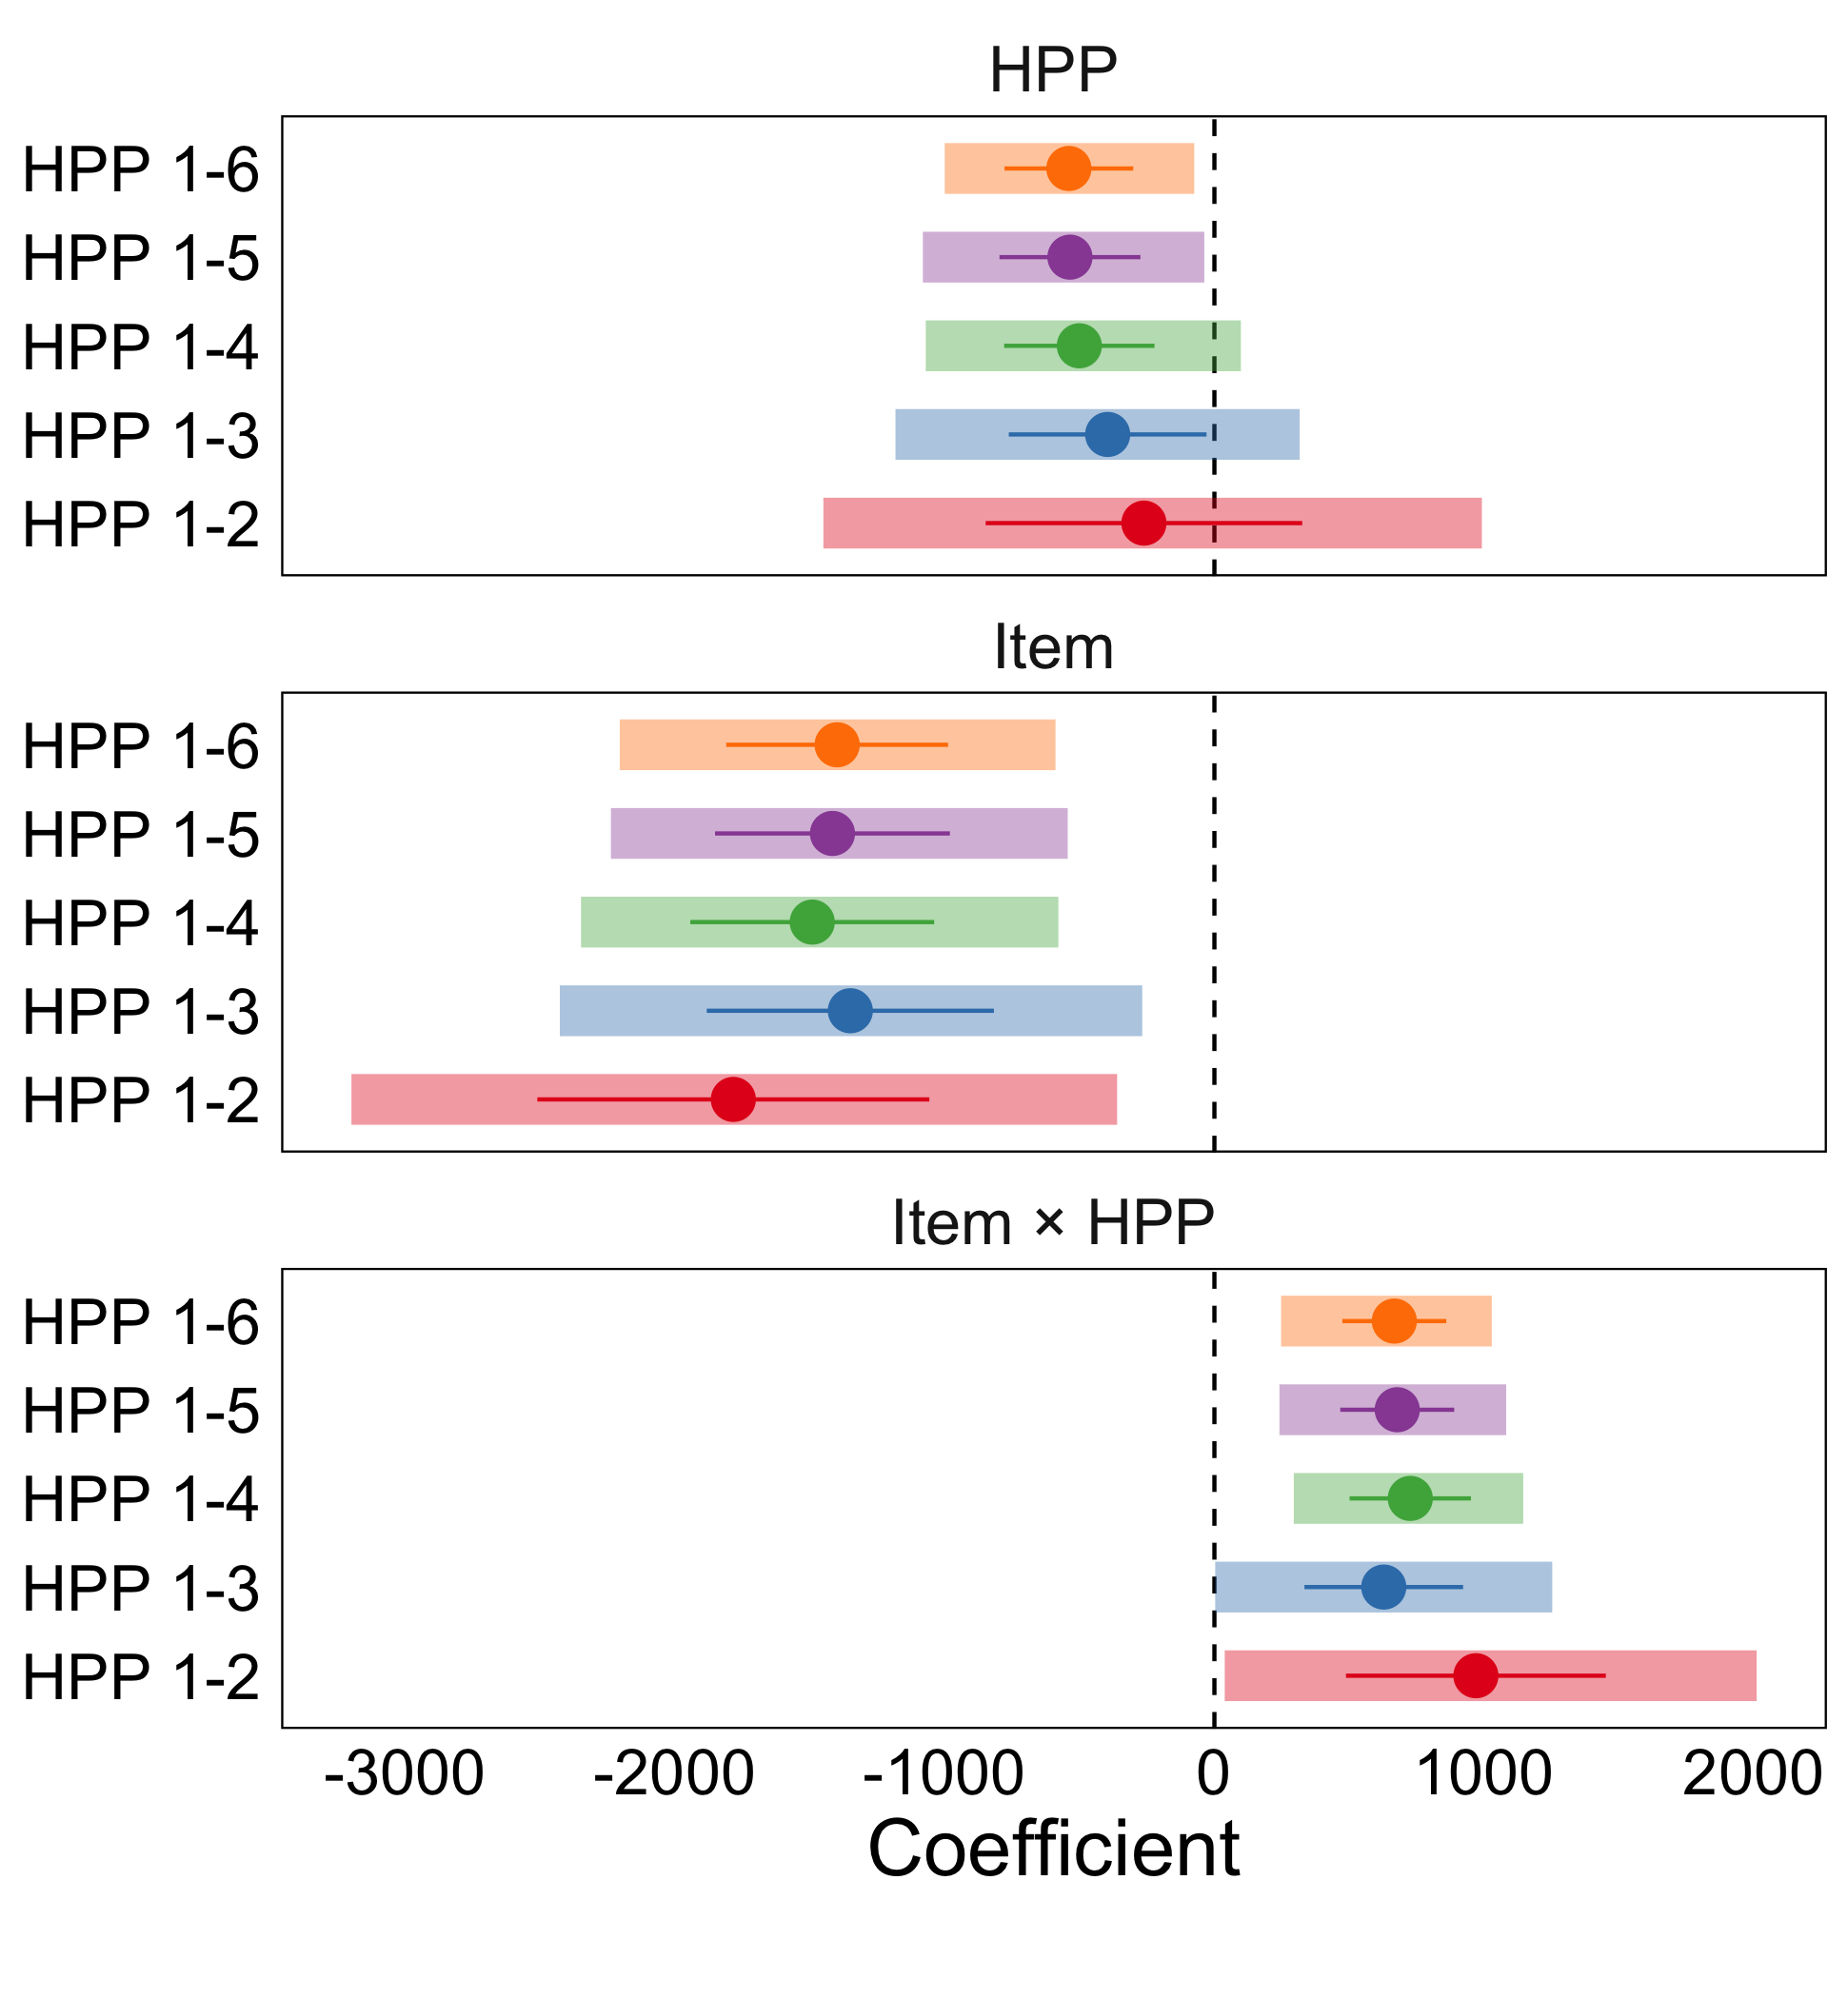
\includegraphics[width=\textwidth]{/home/vant/Documents/Flip/Figures/05_anova-merged} \caption{Estimated coefficients for the three predictors (Test Item, HPP, and their interaction) across the same linear mixed-effects model fitted on the overall sample (HPP 1-6, including all participants), and its subsets (including particpiants that completed less than 6, 5, 4, 3 HPP studies). Dots indicate point estimates, error bars indicate SEs, and shaded boxes indicate 95\% CIs.}(\#fig:unnamed-chunk-18)
\end{figure}

\hypertarget{s5}{%
\subsection{S5: Results of Saffran \& Wilson (2003) and Saffran et
al.~(2008) only}\label{s5}}

We conducted this additional analysis to ensure that the results
obtained on the entire dataset were not driven primarily by the two most
recent datasets (Santolin \& Saffran, 2019; Santolin et al., 2019), in
which we first noticed the pattern of results (i.e., the flip in
preference). Results closely mirrored those of the entire dataset,
showing a statistically significant interaction between test item (novel
vs.~familiar) and number of HPP visits (\emph{F}(1,50.00) = 11.00,
\emph{p} = .002). As shown in the figure below, there is a decline in
familiarity preference as the number of HPP visits increases (Panel A),
and an interaction between test item (novel vs.~familiar) and number of
HPP visits (Panel B).

\begin{figure}
\includegraphics[width=\textwidth]{/home/vant/Documents/Flip/Figures/Older/02_interaction} \caption{A: Difference in looking time between novel and familiar trials for data from Saffran \& Wilson (2003) and Saffran et al. (2008) only, as a function of HPP visits. Shaded bands indicate 95\% CIs. Points represent group means, with error bars representing 95\% CIs. B: Predicted looking time (in ms) for familiar and novel test items plotted against number of HPP visits (older datasets only). Shaded bands represent +1/-1 SEs. Points represent group means with +1/-1 SEs as error bars.}(\#fig:unnamed-chunk-19)
\end{figure}

\hypertarget{s6.-session-info}{%
\subsection*{S6. Session info}\label{s6.-session-info}}
\addcontentsline{toc}{subsection}{S6. Session info}

R version 3.6.3 (2020-02-29) Platform: x86\_64-pc-linux-gnu (64-bit)
Running under: Ubuntu 20.04.1 LTS

Matrix products: default BLAS:
/usr/lib/x86\_64-linux-gnu/blas/libblas.so.3.9.0 LAPACK:
/usr/lib/x86\_64-linux-gnu/lapack/liblapack.so.3.9.0

locale: {[}1{]} LC\_CTYPE=en\_GB.UTF-8 LC\_NUMERIC=C\\
{[}3{]} LC\_TIME=es\_ES.UTF-8 LC\_COLLATE=en\_GB.UTF-8\\
{[}5{]} LC\_MONETARY=es\_ES.UTF-8 LC\_MESSAGES=en\_GB.UTF-8\\
{[}7{]} LC\_PAPER=es\_ES.UTF-8 LC\_NAME=C\\
{[}9{]} LC\_ADDRESS=C LC\_TELEPHONE=C\\
{[}11{]} LC\_MEASUREMENT=es\_ES.UTF-8 LC\_IDENTIFICATION=C

attached base packages: {[}1{]} stats graphics grDevices utils datasets
methods base

other attached packages: {[}1{]} purrr\_0.3.4 kableExtra\_1.2.1
ggplot2\_3.3.2 here\_0.1\\
{[}5{]} tibble\_3.0.3 dplyr\_1.0.2 magrittr\_1.5 knitr\_1.29\\
{[}9{]} papaja\_0.1.0.9997

loaded via a namespace (and not attached): {[}1{]} pillar\_1.4.6
compiler\_3.6.3 highr\_0.8 base64enc\_0.1-3\\
{[}5{]} tools\_3.6.3 digest\_0.6.25 viridisLite\_0.3.0 evaluate\_0.14\\
{[}9{]} lifecycle\_0.2.0 gtable\_0.3.0 pkgconfig\_2.0.3 rlang\_0.4.7\\
{[}13{]} rstudioapi\_0.11 yaml\_2.2.1 xfun\_0.16 xml2\_1.3.2\\
{[}17{]} httr\_1.4.2 withr\_2.2.0 stringr\_1.4.0 generics\_0.0.2\\
{[}21{]} vctrs\_0.3.2 webshot\_0.5.2 rprojroot\_1.3-2 grid\_3.6.3\\
{[}25{]} tidyselect\_1.1.0 glue\_1.4.1 R6\_2.4.1 rmarkdown\_2.3\\
{[}29{]} bookdown\_0.20 backports\_1.1.9 scales\_1.1.1 ellipsis\_0.3.1\\
{[}33{]} htmltools\_0.5.0 rvest\_0.3.6 colorspace\_1.4-1
stringi\_1.4.6\\
{[}37{]} munsell\_0.5.0 crayon\_1.3.4

\hypertarget{references}{%
\subsection*{References}\label{references}}
\addcontentsline{toc}{subsection}{References}

\begingroup
\setlength{\parindent}{-0.5in}
\setlength{\leftskip}{0.5in}

\hypertarget{refs}{}
\leavevmode\hypertarget{ref-barr2013}{}%
Barr, D. J., Levy, R., Scheepers, C., \& Tily, H. J. (2013). Random
effects structure for confirmatory hypothesis testing: Keep it maximal.
\emph{Journal of Memory and Language}, \emph{68}(3), 255--278.
\url{https://doi.org/10.1016/j.jml.2012.11.001}

\leavevmode\hypertarget{ref-bates2015a}{}%
Bates, D., Kliegl, R., Vasishth, S., \& Baayen, H. (2015). Parsimonious
Mixed Models. \emph{arXiv:1506.04967 {[}Stat{]}}. Retrieved from
\url{http://arxiv.org/abs/1506.04967}

\leavevmode\hypertarget{ref-brauer2018}{}%
Brauer, M., \& Curtin, J. J. (2018). Linear mixed-effects models and the
analysis of nonindependent data: A unified framework to analyze
categorical and continuous independent variables that vary
within-subjects and/or within-items. \emph{Psychological Methods},
\emph{23}(3), 389--411. \url{https://doi.org/10.1037/met0000159}

\leavevmode\hypertarget{ref-fox2019}{}%
Fox, J., \& Weisberg, S. (2019). \emph{An R companion to applied
regression} (Third). Thousand Oaks CA: Sage. Retrieved from
\url{https://socialsciences.mcmaster.ca/jfox/Books/Companion/}

\leavevmode\hypertarget{ref-judd2012}{}%
Judd, C. M., Westfall, J., \& Kenny, D. A. (2012). Treating stimuli as a
random factor in social psychology: A new and comprehensive solution to
a pervasive but largely ignored problem. \emph{Journal of Personality
and Social Psychology}, \emph{103}(1), 54--69.
\url{https://doi.org/10.1037/a0028347}

\leavevmode\hypertarget{ref-saffran2008}{}%
Saffran, J., Hauser, M., Seibel, R., Kapfhamer, J., Tsao, F., \&
Cushman, F. (2008). Grammatical pattern learning by human infants and
cotton-top tamarin monkeys. \emph{Cognition}, \emph{107}(2), 479--500.
\url{https://doi.org/10.1016/j.cognition.2007.10.010}

\leavevmode\hypertarget{ref-saffran2003}{}%
Saffran, J. R., \& Wilson, D. P. (2003). From Syllables to Syntax:
Multilevel Statistical Learning by 12-Month-Old Infants. \emph{Infancy},
\emph{4}(2), 273--284. \url{https://doi.org/10.1207/S15327078IN0402_07}

\leavevmode\hypertarget{ref-santolin2019}{}%
Santolin, C., \& Saffran, J. R. (2019). Non-Linguistic Grammar Learning
by 12-Month-Old Infants: Evidence for Constraints on Learning.
\emph{Journal of Cognition and Development}, \emph{20}(3), 433--441.
\url{https://doi.org/10.1080/15248372.2019.1604525}

\leavevmode\hypertarget{ref-santolin2019a}{}%
Santolin, C., Saffran, J. R., \& Sebastian-Galles, N. (2019).
Non-linguistic artificial grammar learning in 12-month-old infants: A
cross-lab replication study. In. Potsdam, Germany.

\endgroup
\end{appendix}
